% journal:APEX
% author:Hiroki Yoshida
\documentclass[10pt]{iopart}
\usepackage{graphicx}
\usepackage{iopams}
\usepackage{bm}
\usepackage{hyperref}


\begin{document}
\title{Magnetoelastic wave in Ferromagnetic Thin-film Mediated by Dipolar Interaction}
% \article{\APEX}{Magnetoelastic wave in Ferromagnetic Thin-film Mediated by Dipolar Interaction}

\author{Hiroki Yoshida$^1$}

\address{$^1$ Department of Physics, Institute of Science Tokyo, Japan}
\ead{yoshida.h.9d8d@m.isct.ac.jp}

\begin{abstract}
    Here comes the abstract ($\leq 200$ words)
\end{abstract}

% \keywords{Universe}
\submitto{\APEX}
\maketitle
\ioptwocol

Hello, world. Main text ($\leq 3200$ words and $\leq 5$ figures, incl. the  Title, Abstract, Main Text, Acknowledgements, References, Tables and figure captions.).

\begin{figure}
    \begin{center}
        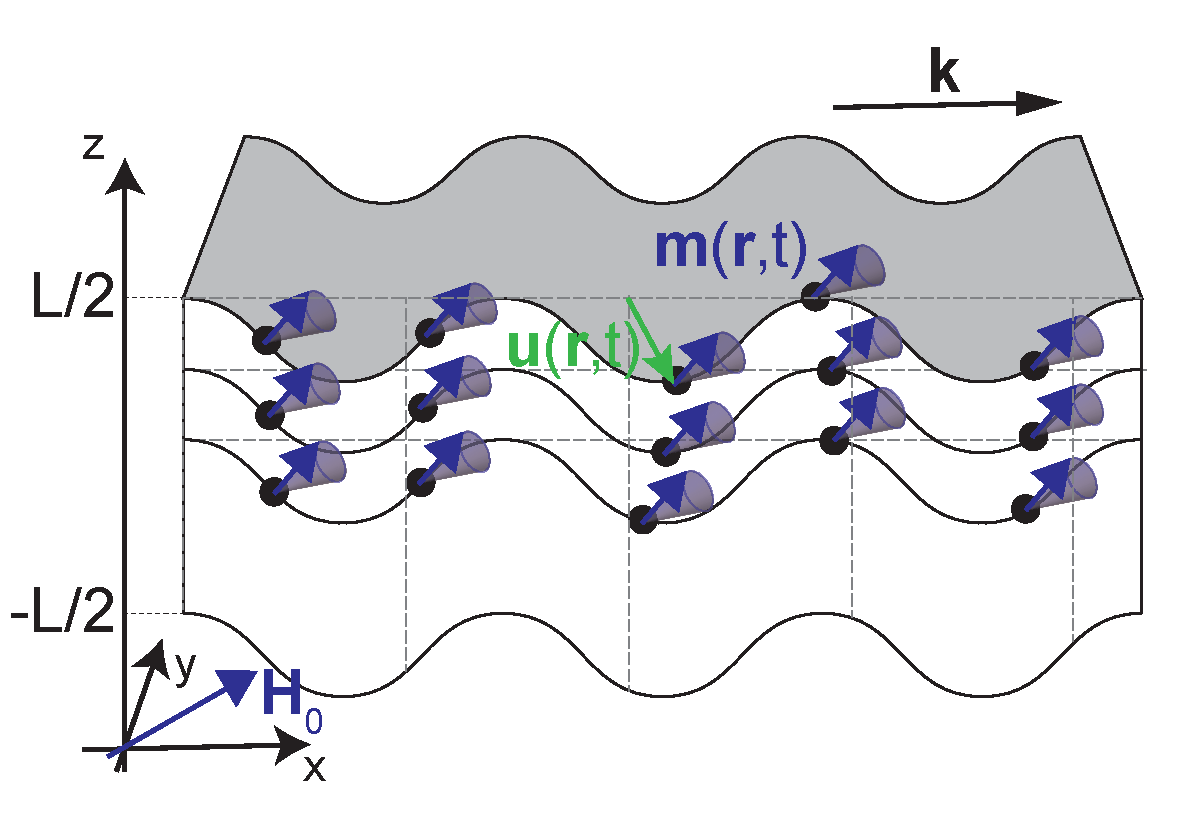
\includegraphics[width=\columnwidth]{fig/Schematic_MSEW.pdf}
        \caption{Schematic illustration of the system under consideration. Ferromagnetic thin-film of thickness $L$ in the $z$ direction and infinitely large in $x$ and $y$ directions. Magnetic moments at each lattice point precess around an axis parallel to the external in-plane magnetic field $\bm{H}_0$. The elastic wave changes positions of magnetic moments and their distance, resulting in the modification of dipolar interaction among them.}
        \label{fig:Schametic}
    \end{center}
\end{figure}

Our system is schematically shown in Fig.~\ref{fig:Schametic}. Consider a ferromagnetic thin film, that is infinitely large in the $xy$ plane and has a finite thickness $L$ in the $z$ direction. The origin is taken to be in the middle of the film. This film is assumed to be isotropic both magnetically and elastically. We apply an in-plane external magnetic field $\bm{H}_0$ to this system. Then, at equilibrium, saturation magnetization $\bm{M}_0$ appear parallel to $\bm{H}_0$. We study the propagation wave of small deviation from equilibrium magnetization $\bm{m}(\bm{r},t)$. This system also has another propagating wave of elastic deformation. At each position $\bm{r}$, the lattice points are shifted by $\bm{u}(\bm{r},t)$. By this deformation, the distance between magnetic dipoles at each lattice point is modulated and the dipole field $\bm{h}(\bm{r},t)$ created by $\bm{m}$ is also affected by $\bm{u}$ and the system shows the elastomagnetic wave propagation. For simplicity, we consider planewaves with frequency $\omega$ and take the $x$ axis parallel to its propagation direction and assume that the system is uniform in the $y$ direction. Then, $\bm{m}$ and $\bm{u}$ can be written as
\begin{equation}
    \bm{m}(\bm{r},t)=\bm{m}(z)e^{i(kx-\omega t)},\\
    \bm{u}(\bm{r},t)=\bm{u}(z)e^{i(kx-\omega t)}.\label{eq:Assumption}
\end{equation}
We study the coupled dynamics of these waves up to the first-order of these quantities. Here, we focus exclusively on the case of in-plane magnetic field. The case of arbitrary external magnetic field will be presented elsewhere.

We start from the basic equations describing the magnetic dipolar interaction: Maxwell's equations. When the elastic deformation is present, the lattice deviates from its equilibrium positions $\bm{r}$ to $\bm{R}:=\bm{r}+\bm{u}(\bm{r},t)$. Then, the Maxwell's equations are rewritten in terms of this new coordinate as
\begin{equation}
    \nabla_{\bm{R}}\cdot \left(\bm{H}+\bm{M}\right)=0,\qquad
    \nabla_{\bm{R}}\times \bm{H}\approx 0,\label{eq:Maxwell_R}
\end{equation}
where in the second equation, the magnetostatic approximation is applied and the time-derivative of electric field is discarded. This approximation is justified when the length scale is long enough so that the dipolar interaction is dominant. We decompose the magnetic field $\bm{H}$ and the magnetization $\bm{M}$ as $\bm{H}=\bm{H}_0+\bm{h}(\bm{r},t)$ and $\bm{M}=\bm{M}_0+\bm{m}(\bm{r},t)$, respectively. Here, $\bm{H}_0$ and $\bm{M}_0$ are quantities at the equilibrium under in-plane external magnetic field and parallel to each other. By the planewave assumptions~(\ref{eq:Assumption}), up to the first-order, the dipolar field can also be written as $\bm{h}=\bm{h}(z)e^{i(kx-\omega t)}$. We rewrite Eq.~(\ref{eq:Maxwell_R}) in terms of these quantities in the original coordinate $\bm{r}$. We note that we need to pay attention to the conservation of the magnetization in a unit volume and as a result we get $\bm{M}(\bm{R})=\bm{M}(\bm{r})/\det(J(\bm{r}))$, where $J(\bm{r})$ is a Jacobi matrix (see Supplemental Material~\cite{SM} for detail). We get
\begin{equation}
    \nabla_{\bm{r}}\cdot\left(\bm{h}(\bm{r})+\bm{m}(\bm{r})\right)=\bm{M}_0\cdot\nabla_{\bm{r}}\left(\nabla_{\bm{r}}\cdot\bm{u}(\bm{r})\right),\label{eq:Maxwell_couple_div}
\end{equation}
\begin{equation}
    \nabla_{\bm{r}}\times\bm{h}(\bm{r})=0,\label{eq:Maxwell_couple_rot}
\end{equation}
where $\nabla_{\bm{r}}$ stands for derivatives with respect to the coordinate $\bm{r}$. Because the surface of the film is also distorted as in Fig.~, boundary conditions to solve these equations are also modified by the existence of $\bm{u}$ as
\begin{equation}
    h^{\mathrm{in}}_x-h_x^{\mathrm{out}}=M_{0,z}\frac{\partial u_z}{\partial x},\label{eq:Maxwell_bc_x}
\end{equation}
\begin{equation}
    h^{\mathrm{in}}_z+m_z-h^{\mathrm{out}}_z=M_{0,x}\frac{\partial u_z}{\partial x},\label{eq:Maxwell_bc_z}
\end{equation}
at $z=\pm L/2$, where $h^{\mathrm{in}/\mathrm{out}}$ stand for the dipolar fields inside and outside of the film, respectively. Following the Green tensor method as in Ref.~\cite{Kalinikos_Slavin_1986}, the dipolar field satisfying Eqs.~(\ref{eq:Maxwell_couple_div}) and (\ref{eq:Maxwell_couple_rot}) under boundary conditions (\ref{eq:Maxwell_bc_x}) and (\ref{eq:Maxwell_bc_z}) is given as (see Seupplemental Material~\cite{SM} for the detail)
\begin{equation}
    \bm{h}(z)=\int_{-\frac{L}{2}}^{\frac{L}{2}}\rmd z'\left(G^m(z,z')\bm{m}(z')+G^u(z,z')\bm{u}(z')\right),\label{eq:dipolar_field}
\end{equation}
where
\begin{equation}
    G^m(z,z')=\left(\begin{array}{ccc}
        -G_P(z,z')&0&-iG_Q(z,z')\\
        0&0&0\\
        -iG_Q(z,z')&0&G_{P'}(z,z')
    \end{array}\right),
\end{equation}
\begin{equation*}
    G^u(z,z')=-ikM_{0,x}G^m(z,z'),\nonumber
\end{equation*}
\begin{equation}
    G_{P}(z,z')=\frac{k}{2}e^{-k|z-z'|},
\end{equation}
\begin{equation}
    G_{Q}(z,z')=\mathrm{sgn}(z-z')G_{P}(z,z'),
\end{equation}
\begin{equation}
    G_{P'}(z,z')=G_{P}(z,z')-\delta(z-z').
\end{equation}
This dipolar field couples the magnetostatic wave and elastic wave on the film. We note that in the current setup, there are no couplings when the equilibrium magnetization is parallel to the $y$ axis, i.e. the external magnetic field is applied in that direction. Otherwise, two waves are coupled via $\bm{h}$.

Next, we examine the effect of the magnetoelastic coupling in the dynamics of the magnetostatic and elastic waves. In the absence of the coupling, the dynamics of magnetization $\bm{m}$ up to its first-order is described by the linearized Landau--Lifshitz equation
\begin{equation}
    \dot{\bm{m}}=-\gamma\left(\bm{m}\times\bm{H}_0+\bm{M}_0\times\bm{h}\right),\label{eq:LandauLifshitz}
\end{equation}
where $\gamma$ is the gyromagnetic ratio. This equation can be derived from a Lagrangian
\begin{equation*}
    L^m[\bm{m},\dot{\bm{m}},\bm{m}^*,\dot{\bm{m}}^*]=\int\rmd z\Re\left[\frac{\mu_0}{4M_0^2\gamma}\bm{M}_0\cdot(\bm{m}\times\dot{\bm{m}}^*)\right.
\end{equation*}
\begin{equation}
    \hspace{2.9cm}\left.-\frac{\mu_0}{4}\left(\bm{h}^*\cdot\bm{h}+\frac{H_0}{M_0}\bm{m}^*\cdot\bm{m}\right)\right].\label{eq:Lagrangian_m}
\end{equation}
We can check it by constructing the Euler--Lagrange equation with respect to $\bm{m}^*$ from this Lagrangian. Here, $\mu_0$ is the vacuum magnetic permeability, which is required to make it consistent with the energy of the magnetic field. On the other hand, the dynamics of the displacement field $\bm{u}$ is described by the Navier--Cauchy equation
\begin{equation}
    \rho\ddot{\bm{u}}=\mu\nabla^2\bm{u}+\left(\mu+\lambda\right)\nabla\left(\nabla\cdot\bm{u}\right),\label{eq:NavierCauchy}
\end{equation}
where $\rho$ is the mass density, $\mu$ and $\lambda$ are Lam\'e constants. The Lagrangian for this equation is
\begin{equation}
    L^u[\bm{u},\dot{\bm{u}},\bm{u}^*,\dot{\bm{u}}^*]=\int\rmd z\left[\frac{\rho}{4}\dot{\bm{u}}^*\cdot\dot{\bm{u}}+\frac{1}{4}\partial_i\sigma_{ij}u_j^*\right],\label{eq:Lagrangian_u}
\end{equation}
where $\sigma_{ij}=\mu(\partial_{i}u_j+\partial_ju_i)+\lambda\delta_{ij}\nabla\cdot\bm{u}$ is the stress tensor. The total Lagrangian of a coupled system is given by the sum of two Lagrangians~(\ref{eq:Lagrangian_m}) and (\ref{eq:Lagrangian_u}). In this case, $\bm{h}$ is no longer just a functional of the amgnetization, but also a functional of the displacement field $\bm{u}$. Therefore, there appear a new volume force term $-\mu_0\bm{f}$ in the Navier--Cauchy equation~(\ref{eq:NavierCauchy}), where the force $\bm{f}$ is given as (see Supplemental Material~\cite{SM} for the detail of derivation)
\begin{equation}
    f_i(z):=\frac{\delta h^*_j}{\delta u^*_i}h_j=-(\bm{M}_0\cdot\nabla)h_i(z).
\end{equation}
Physically, this force can be understood as a Maxwell stress acting on magnetic dipoles at each lattice site caused by the change of the dipolar field, which is induced by the displacement field. The coupled dynamics of the magnetoelastic wave is then given by
\begin{equation}
    \left\{
    \begin{array}{l}
        \dot{\bm{m}}=-\gamma\left(\bm{m}\times\bm{H}_0+\bm{M}_0\times\bm{h}\right)\\
        \rho\ddot{\bm{u}}=\mu\nabla^2\bm{u}+\left(\mu+\lambda\right)\nabla\left(\nabla\cdot\bm{u}\right)-\mu_0\bm{f}.
    \end{array}\label{eq:CoupledEOM}
    \right.
\end{equation}

In order to see the dynamical property of the coupled wave described by the above equations of motion, we numerically calculate the dispersion relation below. By the assumption~(\ref{eq:Assumption}), the time derivative in the left-hand side becomes $-i\omega$. The second equation of Eq.~\ref{eq:CoupledEOM} contains spatial derivative of $\bm{u}$ and requires the boundary condition to solve this equation. Since we consider a film in vacuum, we impose the tension free condition at the surfaces $z=\pm L/2$ as
\begin{equation}
    \sigma_{xz}|_{z=\pm\frac{L}{2}}=\sigma_{yz}|_{z=\pm\frac{L}{2}}=\sigma_{zz}|_{z=\pm\frac{L}{2}}=0.
\end{equation}
Under this condition, a type of elastic wave called Lamb wave appear when the coupling is absent. Since the system is symmetric with respect to the $z=0$ plane, modes of the Lamb wave are either symmetric or anti-symmetric with respect to the sign change of the variable $z$. The magnetostatic wave in this geometry is studied in detail by Damon and Eshbach~\cite{damonMagnetostaticModesFerromagnet1961}. They analytically showed that when the external magnetic field is parallel to the propagation of the wave ($\bm{H}_0\parallel\bm{k}$), the system has infinitely many bulk mode called backward volume wave, which are either symmetric or anti-symmetric. When the magnetic field is in-plane but perpendicular to the propagation ($\bm{H}_0\perp\bm{k}$), there will be a surface mode, which is localized at the surface. For the calculation of the dispersion, it is more convenient to introduce another coordinate $(r_1,r_2,r_3)$, where the original $(x,y,z)$ is rotated around the $z$ axis and $r_1$ axis is taken to be parallel to the external magnetic field. Then, $r_1$ component of $\bm{m}$ is zero since $\bm{M}_0\cdot\dot{\bm{m}}=0$ in the first equation of Eq.~(\ref{eq:CoupledEOM}) and the equation is reduced to an equation about two-component vector $(m_2,m_3)^T$.



\ack{H. Y. Acknowledges support from Japan Society for the Promotion of Science (JSPS) KAKENHI Grant No. JP24KJ1109 and by MEXT Initiative to Establish Next-generation Novel Integrated Circuits Centers (X-NICS) Grant No. JPJ011438. S. M. acknowledges support by Japan Society for the Promotion of Science (JSPS) KAKENHI Grant No. JP22K18687, No. JP22H00108, and No. JP24H02231.}

\bibliographystyle{iopart-num.bst}
\bibliography{Ref_MSEW.bib}

\end{document}